% IMPLEMENTATION
\chapter{Implementation}\label{chapter:implementation}

\section{Data model}\label{section:datamodel}

To structure the information on the level of the data, different alternatives can be conceived to represent the data made available through the public API. For example, conversations can be represented as \texttt{XML}, as shown in listing \ref{listing:xmldb}. Operations can then be implemented to append or remove elements.

%% LISTING
\lstinputlisting[language=XML, caption={Example of an \texttt{XML} data representation.}, label={listing:xmldb}]{code/database.xml}

Alternatively, a NoSQL database can be designed, for example using the Datastore on Google App Engine (GAE).

For this application, a relational database was implemented using \texttt{MySQL}. Figure \ref{figure:erd} shows the entity relationship diagram (ERD) of the entities in the database. As the backend of the application was created with \texttt{PHP}, \emph{PHPMyAdmin}\footnote{\url{http://www.phpmyadmin.net/home_page/index.php}} was used to create the database.

\begin{figure}
	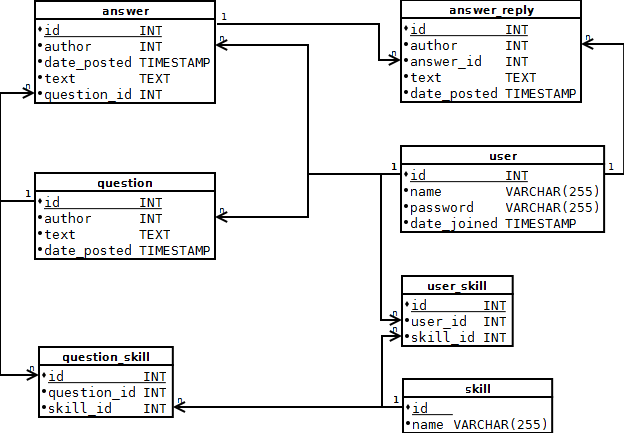
\includegraphics[width=400px]{img/erd}
	\caption{Entity relationship diagram of the database.}
	\label{figure:erd}
\end{figure}

\subsection{Remarks}

Although the relational database certainly will do the job in this case, under certain conditions NoSQL databases scale better when huge quantities of data are involved. As a result, if this app would be used by a great number of students, it is not unlikely that another design choice may outperform this one.



% REST
\section{Server}
% php (alternative google app engine)

The REST API is implemented using the codeigniter framework. Codeigniter\footnote{\url{http://ellislab.com/codeigniter}} is a \texttt{PHP} framework that relies heavily on the model-view-controller design principles. Via model classes the database can be accessed. Controllers can load model classes to pass on the data to the views. A special controller, \texttt{Api}, which extends the \texttt{REST\_Controller}\footnote{The source code can be found at \url{https://github.com/philsturgeon/codeigniter-restserver}} class, implements the REST service.

Each method listed in table \ref{table:rest_api} is then implemented in the \texttt{Api} class. Each method signature has as a suffix an underscore followed by the HTTP method name, e.g. for the method \emph{create} and HTTP method POST, this results in \emph{create\_post}. The class diagram of the backend of the application is shown in figure \ref{figure:codeigniter:classdiagram}. Figure \ref{figure:architecture:global2} summarize the application's internal structure as discussed so far.

%% class codeigniter
\begin{figure}
	\begin{center}
		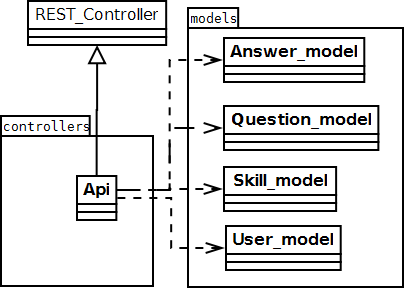
\includegraphics[width=200px]{img/codeigniter_class_diagram}
		\caption{The class diagram of the codeigniter project.}
		\label{figure:codeigniter:classdiagram}
	\end{center}
\end{figure}


%% global2
\begin{figure}
	\begin{center}
		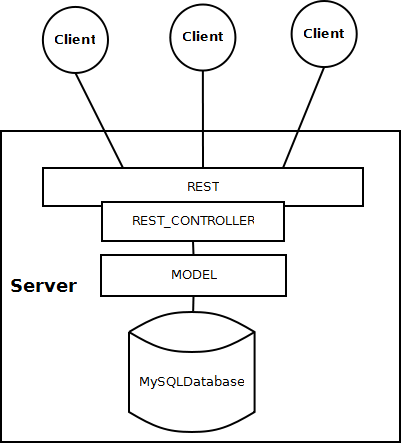
\includegraphics[width=200px]{img/architecture_global2}
		\caption{The global architecture of the application, including REST, the Codeigniter MVC design and the MySQL database.}
		\label{figure:architecture:global2}
	\end{center}
\end{figure}

Alternative libraries for REST and PHP exist, but also for other technologies, such as GAE. For example the Boomi Appengine REST Server\footnote{\url{https://code.google.com/p/appengine-rest-server/}} is a library for Google App Engine applications. Of course, this would also require a somewhat different underlying data model as mentioned earlier.

\subsection{Remarks}

When designing an API as described above, it is important to ensure that the data remains consistent. In this case, the login functionality forms a possible danger in that respect, as a user may log in from multiple apps simultaneously, and the server doesn't keep track of the number of logged in apps per user account. At the moment the session key is required to ensure that no one else log out any other user. Instead, a solution might be to create a separate table to keep track of these sessions, rather than keep a single session key entry in the user table.

If we were to create only the mobile web app, which depending on the type of application, is quite reasonable, implementing a REST API may seem like overkill. Instead a simpler design could be used to persist data. Nonetheless, when developing multiple native applications, the cost savings of creating a back-end to process parts of the data may be significant. For example, graphical operations that require a lot of computational power may be done on the device itself, while operations on the data may be done on the server.

Coming back to the point raised earlier on the performance bottleneck of a relational database. Suppose this is the case, having a well-defined API provides transparency, as the clients depend on the public interface, rather than how everything works under the hood.



\section{Clients}

Now that we have discussed the server side of the architecture, we will take a closer look at the different clients. For this project, very few code was actually written at the client side. Eventually it has become merely an experiment to test the client-server architecture, rather than an elaborate implementation of the application as described in chapter \ref{chapter:requirement_analysis}. Nonetheless, we will focus further on how the final elements of the architecture fall into place for each app.


\subsection{HTML5 mobile web application}

The \texttt{HTML5} mobile web application is basically implemented as an \texttt{HTML} web page enhanced with the jQuery mobile library\footnote{\url{http://jquerymobile.com/}}. The internal architecture consists out of JavaScript, HTML and CSS. The JavaScript code consists out of a number of libraries and source code making the connection to the back-end and controlling the view. The jQuery mobile library provides a layer on top of the original JavaScript to facilitate operations for modifying the view and the use of AJAX. A second library mirrors the REST API methods and helps to provide additional transparency when making asynchronous calls to the server. The resulting application structure is shown in figure \ref{figure:html5:architecture}.

%% architecture HTML5
\begin{figure}
	\begin{center}
		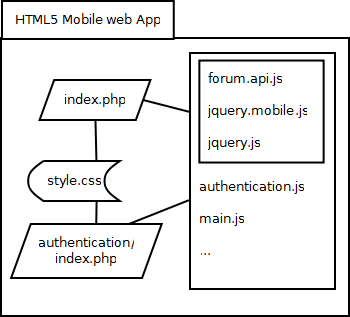
\includegraphics[width=200px]{img/html5_architecture}
		\caption{The internal structure of the HTML5 mobile web app.}
		\label{figure:html5:architecture}
	\end{center}
\end{figure}


Listing \ref{listing:html5:api} shows how the connection is made to the server in the api library. Listing \ref{listing:html5:api:use} shows how it is used in the application. An asynchronous call is made to the server. Once the result is available the anonymous function on line 5 to 13 in listing \ref{listing:html5:api:use} is executed.

\lstinputlisting[language=Java, firstline=1, lastline=16, caption={A method from the JavaScript API library to make the connection to the server.}, label={listing:html5:api}]{code/forum.api.js}

\lstinputlisting[language=Java, firstline=1, lastline=15, caption={Calling a method from the JavaScript API library.}, label={listing:html5:api:use}]{code/authentication.js}


\subsection{Android application}

The Android application follows a similar design. A seperate collection of classes provides transparent access to the REST methods of the server, as shown in figure \ref{figure:android:architecture}. Instead of passing an anonymous function as parameter, a specific listener is implemented for each asynchronous operation. Once the data is available, the notify method of the listener is called. The custom implementation of this method deals with the result from the request. This is shown in listings \ref{listing:android:api}, \ref{listing:android:listener} and \ref{listing:android:activity}. The corresponding class diagram is shown in figure \ref{figure:android:classdiagram}.

%% architecture Android
\begin{figure}
	\begin{center}
		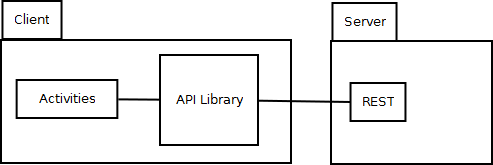
\includegraphics[width=300px]{img/android_architecture}
		\caption{The internal structure of the Android native app.}
		\label{figure:android:architecture}
	\end{center}
\end{figure}

\lstinputlisting[language=Java, firstline=6, lastline=36, caption={AnsyncTask to execute an asynchronous request to the REST server.}, label={listing:android:api}]{code/Authentication.java}

\lstinputlisting[language=Java, firstline=1, lastline=3, caption={Listener for the StartSession task.}, label={listing:android:listener}]{code/StartSessionListener.java}

\lstinputlisting[language=Java, firstline=1, lastline=15, caption={Activity that implements the StartSession listener.}, label={listing:android:activity}]{code/MainActivity.java}

%% class diagram Android
\begin{figure}
	\begin{center}
		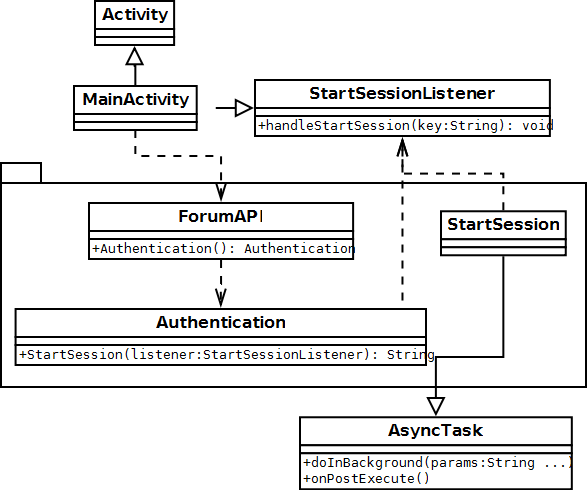
\includegraphics[width=350px]{img/android_class_diagram}
		\caption{Class diagram for the Android app.}
		\label{figure:android:classdiagram}
	\end{center}
\end{figure}


\subsection{iOS application}

Unfortunately no implementation for iOS has been completed. The global structure of the class diagram for the application would have been relatively similar to the Android application, cf. figure \ref{figure:android:architecture}, again with a separate library, which can be implemented in iOS through a static library\footnote{\url{https://developer.apple.com/library/ios/technotes/iOSStaticLibraries/Introduction.html}}, or model classes that are mapped onto the REST service's resources.

To work with REST on iOS, the RESTKit\footnote{\url{http://restkit.org/}; a recent tutorial can be found here: \url{http://www.raywenderlich.com/13097/intro-to-restkit-tutorial}} library can be used for this purpose.



